\section{RITAS algorithm}

Our algorithm constructs yield maps through the following steps:
Rectangle creation, Intersection assignment, Tesselation,
Apportioning, and Smoothing (RITAS). The overarching goal of this
process is to mimic the real world harvesting processes. Figure
\ref{algoplots} provides an illustration of these steps.

\begin{figure}[h!]  \centering
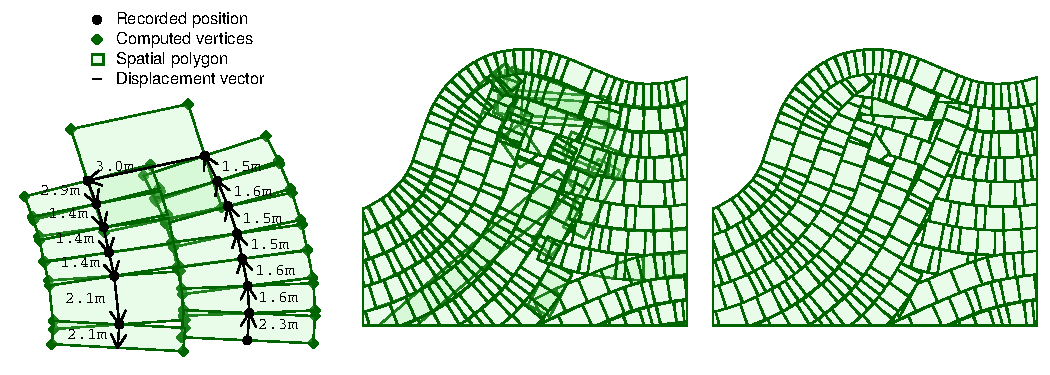
\includegraphics[width=\textwidth]{algoplots}
    \caption{Close-up illustration of some of the pre-processing
steps. \underline{Left}: construction of the vehicle polygons from the
GPS location data. Black dots mark the location at the end of each
logging cycle, green dots correspond to the vertices computed
according to the displacement vector implied by two consecutive
spatial points. The distance traveled could be reported by the yield
monitor or estimated from the vector length. \underline{Center}:
spatial polygons reveal overlap (darker areas) due to driving
maneuvers. \underline{Right}: clipping eliminates the overlap by
assigning intersecting areas to the first polygon in time.}
    \label{fig:closeup}
\end{figure} \TODO{FIGURE 1: Replace with the version JN sketched,
scanned, and emailed.}

Each precision yield data set is assumed to have time-ordered rows
containing the following information: mass harvested $m_t$,
2-dimensional spatial coordinate $(x_t,y_t)$, and swath width $2w_t$
(so that $w_t$ represents the half-width) for $t=0,\ldots,T$.  We
assume any lag time has been effectively pre-processed by
appropriately matching the mass harvested to its 2-dimensional
location.  \JN{Add reference to techniques to do this.}

\subsubsection*{Step 1: Rectangle creation}

Figure \ref{} illustrations the construction of a rectangular
representing the harvested area between each sequential pair of
spatial coordinates. To construct this rectangle, we draw a line
segment from the current coordinate to the previous coordinate with
slope $s_t = (y_t-y_{t-1})/(x_t-x_{t-1})$.  The rectangle is then
constructed according to the area a new line segment of length equal
to the swath width, centered on the first line segment, and with slope
$s'_t = -1/s_t$, would sweep out as it progresses from the previous
coordinate to the current coordinate.  The rectangle associated with
mass $m_t$ has these vertices: $\{(x_{t-1} + d_t, y_{t-1} +
d_ts'_t),(x_{t-1} - d_t, y_{t-1} - d_ts'_t), (x_{t } + d_t, y_{t } +
d_ts'_t),(x_{t } + d_t, y_{t } + d_ts'_t)\}$ where $d_t =
tan^{-1}(s'_t)$.  This step creates $T$ rectangles covering the
harvested area each with an associated mass of harvested crop.

\paragraph{Step 2: Intersection assignment.}  Figure \ref{} shows end
result of this rectangle construction which produces rectangles will
overlap, an area called the \emph{intersection}, due to adjacent
harvester paths.  These intersections are assigned to the first
rectangle, but removed from any later rectangles creating new
polygons.  This step creates $T$ polygons which partition the
harvested area.  Each polygon is associated with the same mass it had
in Step 1, but now the area may be smaller (due to the intersection
removal) and thus yield is more accurately captured.

\paragraph*{Step 3: Tessellation and Apportioning} To aid spatial
smoothing and year-over-year analyses, a regular tesselation of the
harvested area is constructed.  While any tile could work, we
generally use squares, i.e. gridding, with a small size, e.g. $9 m^2$.
Figure \ref{} provides an example tesselation covering the harvested
area.

Mass is apportioned from the polygons of Step 2 to tiles in the
tessellation according to their proportion of the total polygon
area. Where tiles overlap multiple polygons, the tiles receive mass
from each of the polygons according to the area of overlap relative to
each polygon's area.  Thus, the mass associated with the $n$th tile is
$m_n^* = \sum_{t=1}^T p_{t,n} m_t$ where $p_{t,n}$ is the proportion
of polygon $t$'s area in the intersection of polygon $t$ and tile $n$.
This step creates $N$ polygons, determined by the user based on
tesselation resolution, partitioning the harvested area each with an
associated mass of harvested crop.

\paragraph{Step 4: Smoothing} Figure \ref{} shows the regular
tesselation with apportioned mass.  The regular tesselation provides
constant areas and meaningful centroids, and therefore we can use
standard spatial smoothing techniques directly on mass, as opposed to
yield.  We smooth using a Gaussian Process (GP) with a Mat\'ern
covariance on the logarithm of mass
\citep{handcock1993bayesian,gutt2006studies}.  Compared with the more
common powered exponential covariance functions, e.g. Gaussian or
exponential, the Mat\'ern adds an additional parameter that controls
local smoothness, i.e. \ differentiability, and therefore is often more
accurate for real world processes.

Covariance parameters are estimated, and smoothed values are found for
each tile following \cite{Cressie1993}.  Specifically, for each tile
we have a predicted mean $\hat\mu_{\ell}$ and variance
$\hat\sigma^2_{\ell}$ for the logarithm of mass.  We using the
following formulas to convert back to the mean and variance of mass
\[ \hat{\mu}_{m} = \exp\left(\hat{\mu}_{\ell} +
\hat{\sigma}^2_{\ell}/2\right), \quad\mbox{and}\quad
\hat{\sigma}^2_{m} = \exp\left(2 \hat{\mu}_{\ell} +
\hat{\sigma}^2_{\ell}\right)
\left[\exp\left(\hat{\sigma}^2_{\ell}\right) - 1\right].
 \] Finally, yield is calculated by dividing the tile mass by the tile
area.  Figure \ref{} provides smoothed version of Figure \ref{}.

\subsection{Protocol assessment}

One appealling aspect of our approach is that data are not eliminated
based on arbitrary thresholds.

\JN{What percentage of observations did we throw out?  Vega used R,
can we compare to running his algorithm on our data.}

\JN{Variogram}

\LD{Correlation Yield, TWI for YM raw data vs aggregated vs smoothed}

%%% Local Variables:
%%% mode: latex
%%% TeX-master: t
%%% End:
